\begin{Code}
---------------------------------- python ----------------------------------
>>> romc.sample(n2)
----------------------------------------------------------------------------
\end{Code}

\noindent
This is the basic inference utility of the ROMC implementation; we
draw \(n_2\) samples for each bounding box region. This gives a total of
\(k \times n_2\), where \(k < n_1\) is the number of the optimal points
remained after filtering\footnote{From the \(n_1\) optimisation
  problems, only the ones with \(d_i(\thetab^*) < \epsilon\) are
  maintained for building a bounding box}. The samples are drawn from
a uniform distribution \(q_i\) defined over the corresponding bounding
box and the weight \(w_i\) is computed as in
Algorithm~\ref{alg:sampling_GB}.

\begin{Code}
---------------------------------- python ----------------------------------
>>> romc.compute_expectation(h) # E[h(x)|theta]
>>> romc.eval_unorm_posterior(theta, eps_cutoff=False) # unnorm p(theta)
>>> romc.eval_posterior(theta, eps_cutoff=False) # normalised p(theta)
----------------------------------------------------------------------------
\end{Code}

\noindent
The function \code{compute_expectation} computes the expectation
\(\E_{p(\thetab|\data)}[h(\thetab)]\) using
expression~\eqref{eq:expectation}. The argument \code{h} can be any
python \code{Callable}. The method \code{eval_unnorm_posterior} computes
the unnormalised posterior approximation using the
expression~\eqref{eq:approx_posterior}. The method \code{eval_posterior}
evaluates the normalised posterior estimating the partition function
\(Z = \int p_{d,\epsilon}(\thetab|\data)d\thetab\); with Riemann's
integral approximation. The approximation is computationally feasible
only in a low-dimensional parametric space.

\subsubsection*{Example - Sampling and compute expectation}

In the following code snippet, we use the inference utilities to (a)
get weighted samples from the approximate posterior, (b) compute an
expectation and (c) evaluate the approximate posterior. We also use
some of \pkg{ELFI}'s built-in tools to get a summary of the obtained
samples. For the utility \code{compute_expectation}, we demonstrate
how to use it in order to compute the samples mean and
variance. Finally, we evaluate \code{eval_posterior} at multiple
points to plot the approximate posterior of
Figure~\ref{fig:running_example_romc_inference}. We observe that the
approximation is quite close to the ground-truth.

\begin{Code}
------------------------------ python snippet ------------------------------  
  # Inference part
  seed = 21
  n2 = 50
  romc.sample(n2=n2, seed=seed)

  # visualize region, adding the samples now
  romc.visualize_region(i=1)

  # Visualise marginal (built-in ELFI tool)
  romc.result.plot_marginals(weights=romc.result.weights,
                             bins=100, range=(-3,3))

  # Summarize the samples (built-in ELFI tool)
  romc.result.summary()
  # Number of samples: 19300
  # Sample means: theta: -0.0116

  # compute expectation
  exp_val = romc.compute_expectation(h=lambda x: np.squeeze(x))
  print("Expected value   : %.3f" % exp_val)
  # Expected value   : -0.012

  exp_var = romc.compute_expectation(h=lambda x: np.squeeze(x)**2)
  print("Expected variance: %.3f" % exp_var)
  # Expected variance: 1.120

  # eval unnorm posterior
  romc.eval_unnorm_posterior(theta=0)

  # check eval posterior
  romc.eval_posterior(theta=0)
----------------------------------------------------------------------------
\end{Code}

% \begin{figure}[h]
%     \begin{center}
%       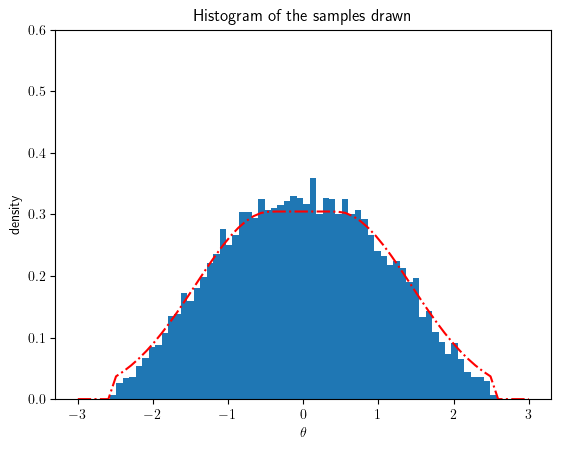
\includegraphics[width=0.48\textwidth]{./latex_files/images/chapter3/example_marginal.png}
%     \end{center}
%   \caption[Histogram of the obtained samples at the 1D example.]{(a) Left: Histogram of the obtained samples. (b) Right: Acceptance region around \(\theta_1^*\) with the obtained samples plotted inside.}
%   \label{fig:example_sampling}
% \end{figure}

% \begin{figure}[h]
%     \begin{center}
%       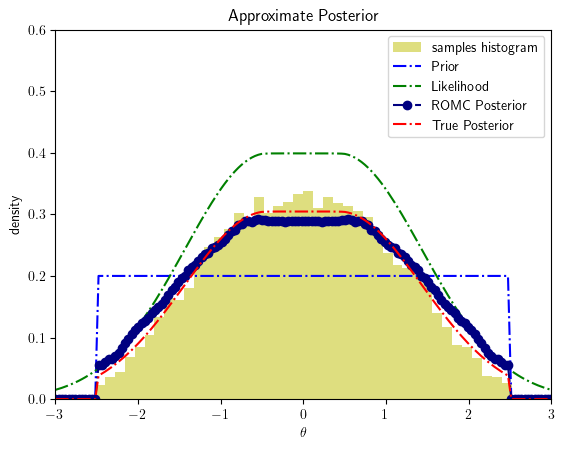
\includegraphics[width=0.6\textwidth]{./latex_files/images/chapter3/example_posterior.png}
%     \end{center}
%   \caption[Approximate posterior evaluation, at the 1D example.]{Approximate posterior evaluation.}
%   \label{fig:approx_posterior}
% \end{figure}
